% TEXINPUTS=.:$HOME/git/bvtex: latexmk  -pdf <main>.tex
\documentclass[xcolor=dvipsnames]{beamer}

\input{defaults}
\input{beamer/preamble}

\setbeamertemplate{navigation symbols}{}
% \setbeamertemplate{background}[grid][step=1cm]

\usepackage{siunitx}
\usepackage{xmpmulti}
\usepackage[export]{adjustbox}

\usepackage[outline]{contour}
\usepackage{tikz}
\usetikzlibrary{shapes.geometric, arrows}
\usetikzlibrary{positioning}

\definecolor{bvtitlecolor}{rgb}{0.98, 0.92, 0.84}
\definecolor{bvoutline}{rgb}{0.1, 0.1, 0.1}

\renewcommand{\bvtitleauthor}{Brett Viren}
\renewcommand{\bvtitle}{\LARGE LARF Status\\{\small 3D Field and Detector Response Calculations}}
\renewcommand{\bvtit}{LARF Status}
\renewcommand{\bvevent}{\Large BNL-DUNE\\\today}
\renewcommand{\bvbeamerbackground}{}

\newcommand{\microboone}{MicroBooNE\xspace}


\begin{document}
\input{beamer/title.tex}
\input{beamer/toc.tex}

\section{Parallel Wires}

\begin{frame}
  \frametitle{Parallel Wires for ``Fake'' 2D}
  \begin{columns}
    \begin{column}{0.4\textwidth}
      \begin{center}
        \includegraphics[width=\textwidth]{twodee-fine-x.pdf}

        \includegraphics[width=0.7\textwidth]{twodee-fine-z.pdf}
      \end{center}
    \end{column}
    \begin{column}{0.4\textwidth}
      \begin{center}
        \includegraphics[width=\textwidth]{twodee-fine-iso.pdf}

        \includegraphics[width=0.7\textwidth]{twodee-fine-y.pdf}
      \end{center}
    \end{column}
  \end{columns}
\end{frame}


\begin{frame}
  \frametitle{Parallel Wires - Slice Through Weighting Potentials}
  \begin{columns}
    \begin{column}{0.3\textwidth}
      \begin{center}
        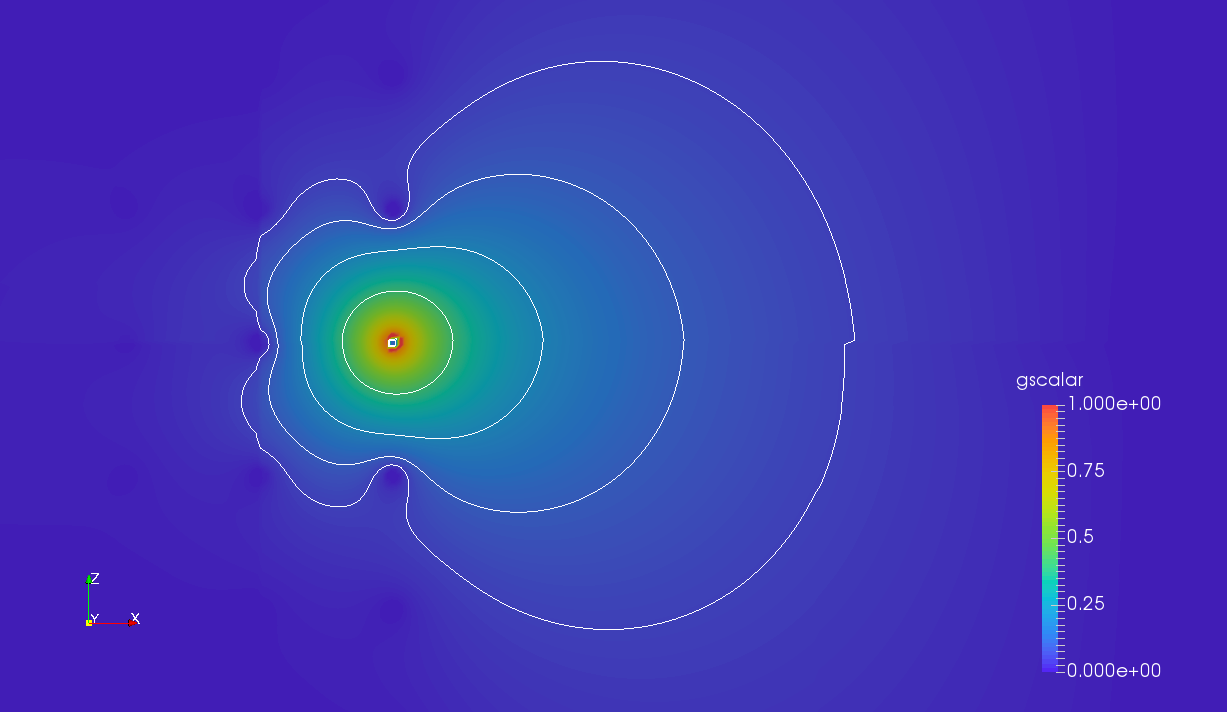
\includegraphics[height=2cm]{twodee-fine-u7.png}

        \scriptsize U plane
      \end{center}
    \end{column}
    \begin{column}{0.3\textwidth}
      \begin{center}
        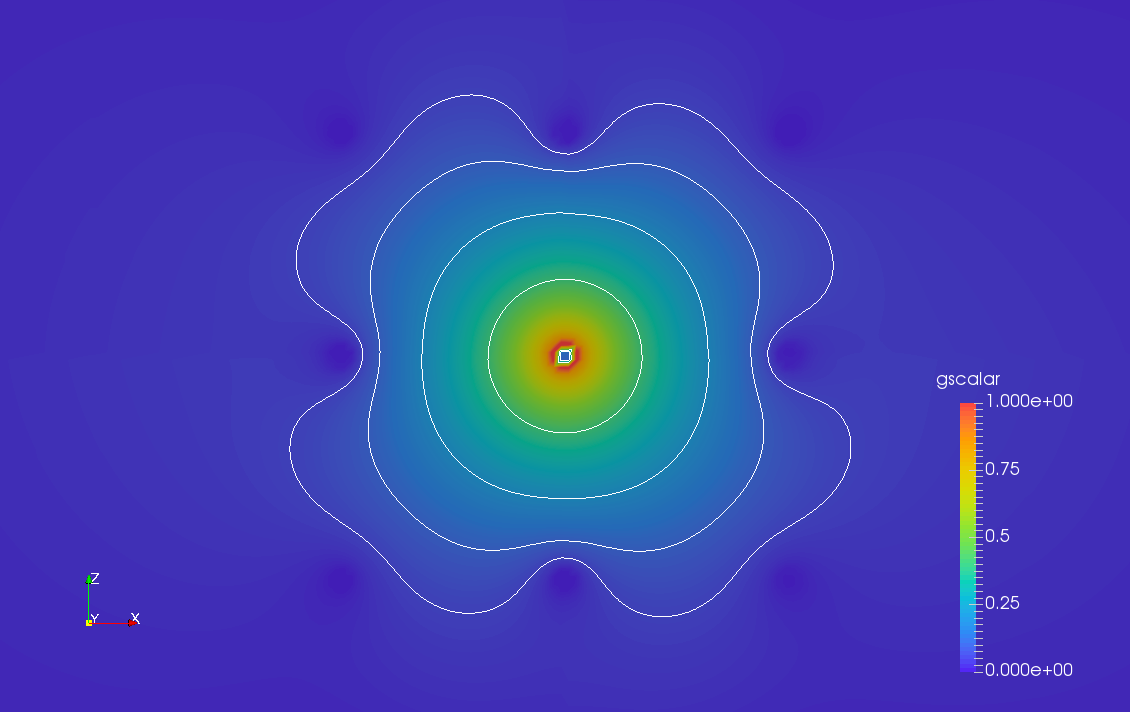
\includegraphics[height=2cm]{twodee-fine-v7.png}
        
        \scriptsize V plane
      \end{center}
    \end{column}
    \begin{column}{0.3\textwidth}
      \begin{center}
        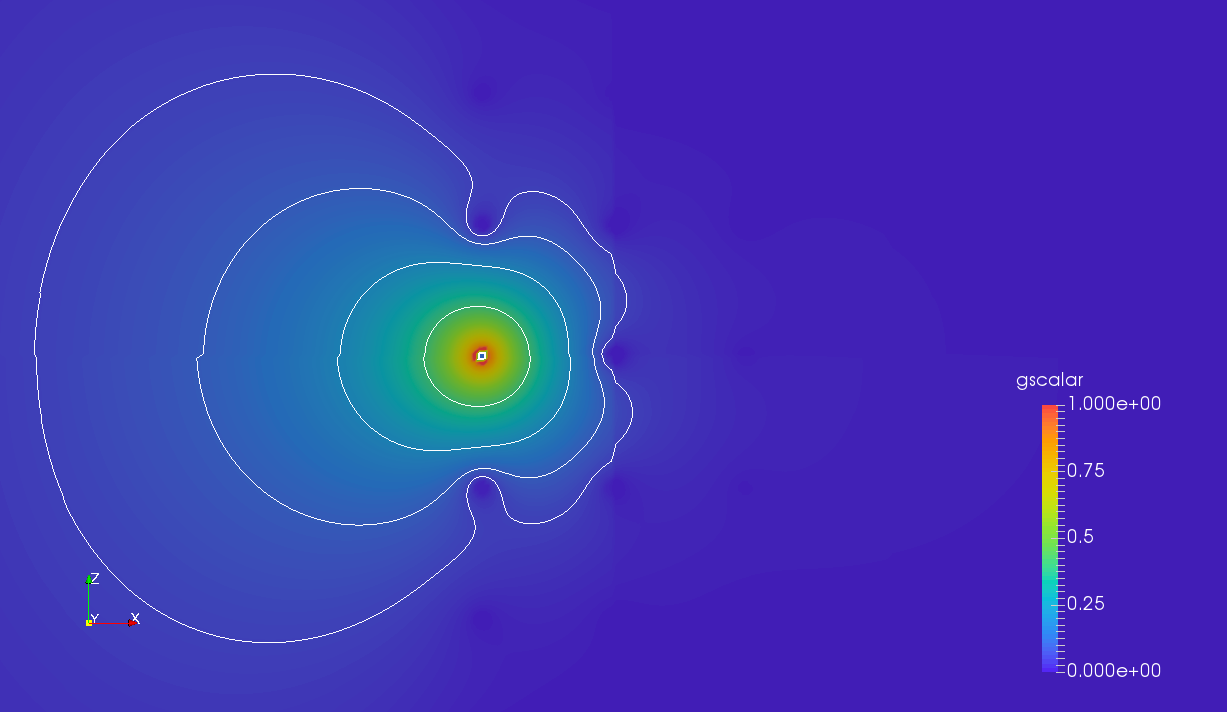
\includegraphics[height=2cm]{twodee-fine-w7.png}

        \scriptsize W plane
      \end{center}
    \end{column}
  \end{columns}

  \begin{itemize}\footnotesize
  \item X-Z slice through plane of symmetry (Y=0).
  \item Color shows weighting potential: 0-100\%.
  \item Lines: 5\%, 10\%, 20\%, 40\% weights.
  \item Gaussian quadrature imprecision visible in some jaggy contous lines.
  \item Small spatial fluctuations near wires, but somewhat obscured.
    \begin{itemize}\scriptsize
    \item Note: inside wire is $\sim$0V, square shape is pixelization.
    \end{itemize}
  \end{itemize}

  \begin{center}
    Visual comparison with Bo's 2D fields show good agreement.

    For now, consider this enough validation to move forward.
  \end{center}
\end{frame}

\section{MicroBooNE Geometry}

\begin{frame}
  \frametitle{Where I'm at}
  \begin{itemize}
  \item MicroBooNE geometry
  \item 20mm patch of wire planes + single plane providing applied potential.
  \item 3D potentials: drift + weight for middle U, V and W wires
  \item Coarse 0.5mm voxel field evaluations spanning +/- 20mm
  \item Fine 0.1mm voxel field evaluations spanning +/- 5mm
  \item Can step in \texttt{paraview} for display
  \item Can step in my code to collect current waveforms.
  \end{itemize}
\end{frame}


\begin{frame}
  \frametitle{Wire Geometry with Cathode Plane}
  \begin{columns}
    \begin{column}{0.5\textwidth}
      \begin{center}
        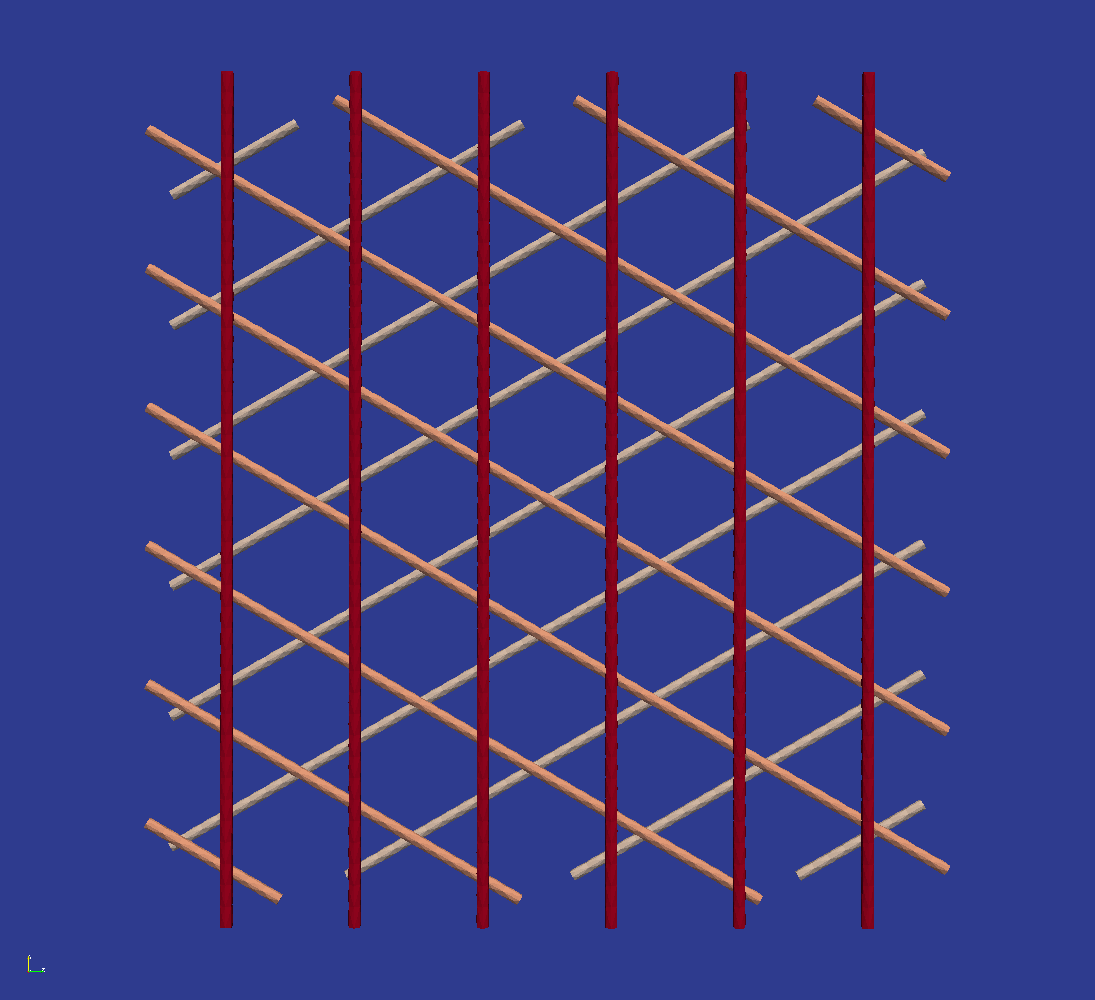
\includegraphics[width=\textwidth]{wires-flat.png}
      \end{center}
    \end{column}
    \begin{column}{0.5\textwidth}
      \begin{center}
        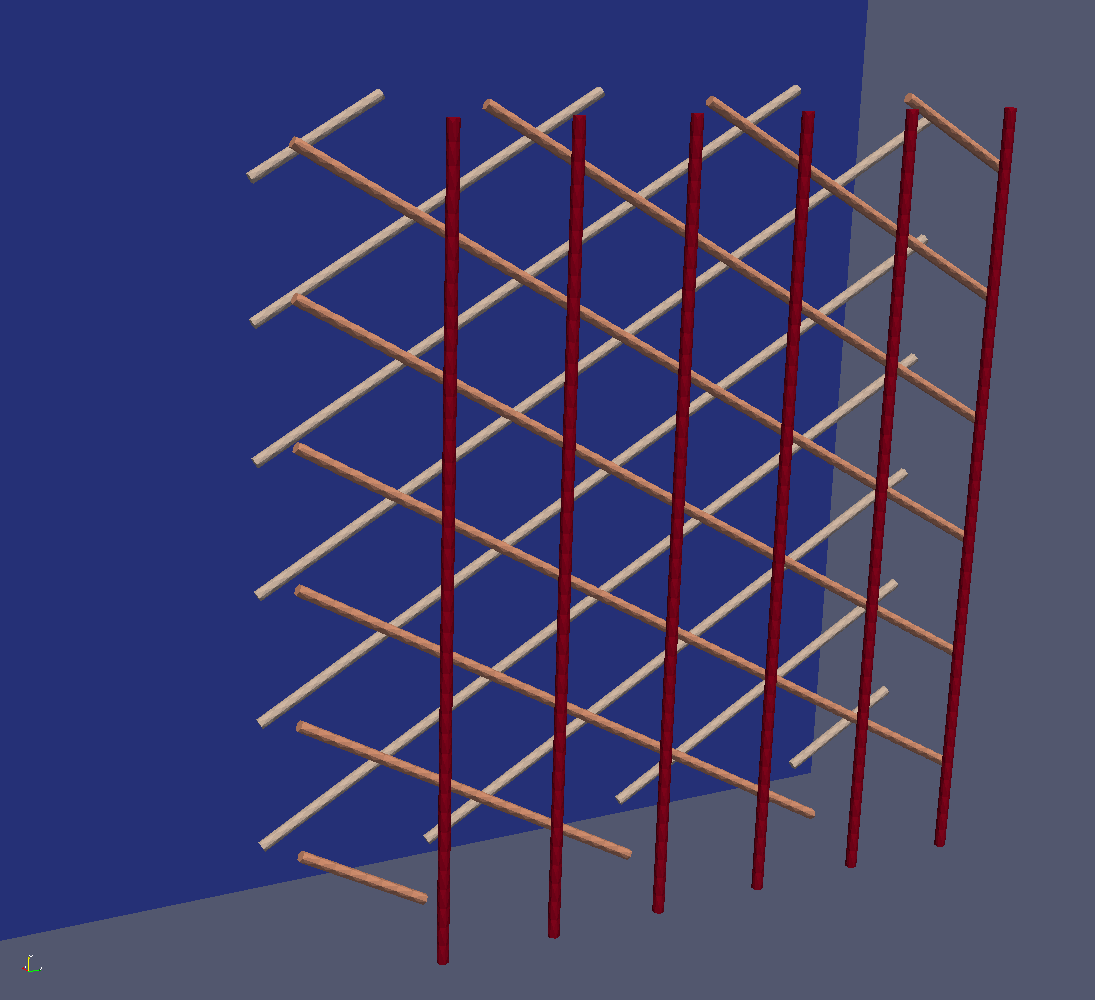
\includegraphics[width=\textwidth]{wires-iso.png}
      \end{center}
    \end{column}
  \end{columns}
  
\end{frame}

\begin{frame}
  \frametitle{U weighting field slices}
  \begin{center}
      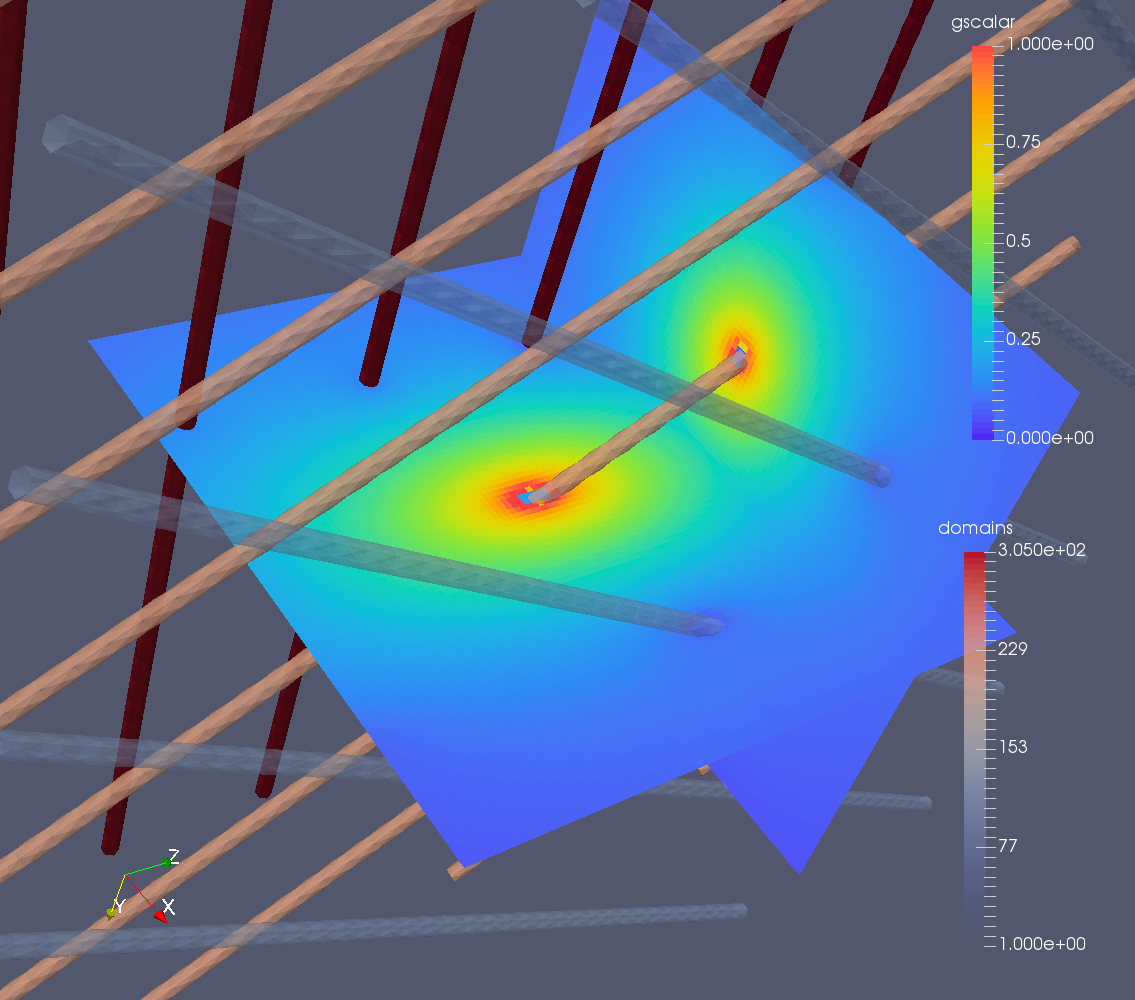
\includegraphics[width=0.7\textwidth]{cap-vweight-field-fine-slices.png}
  \end{center}
\end{frame}

\begin{frame}
  \frametitle{Paraview stepping from line source}
  \begin{center}
      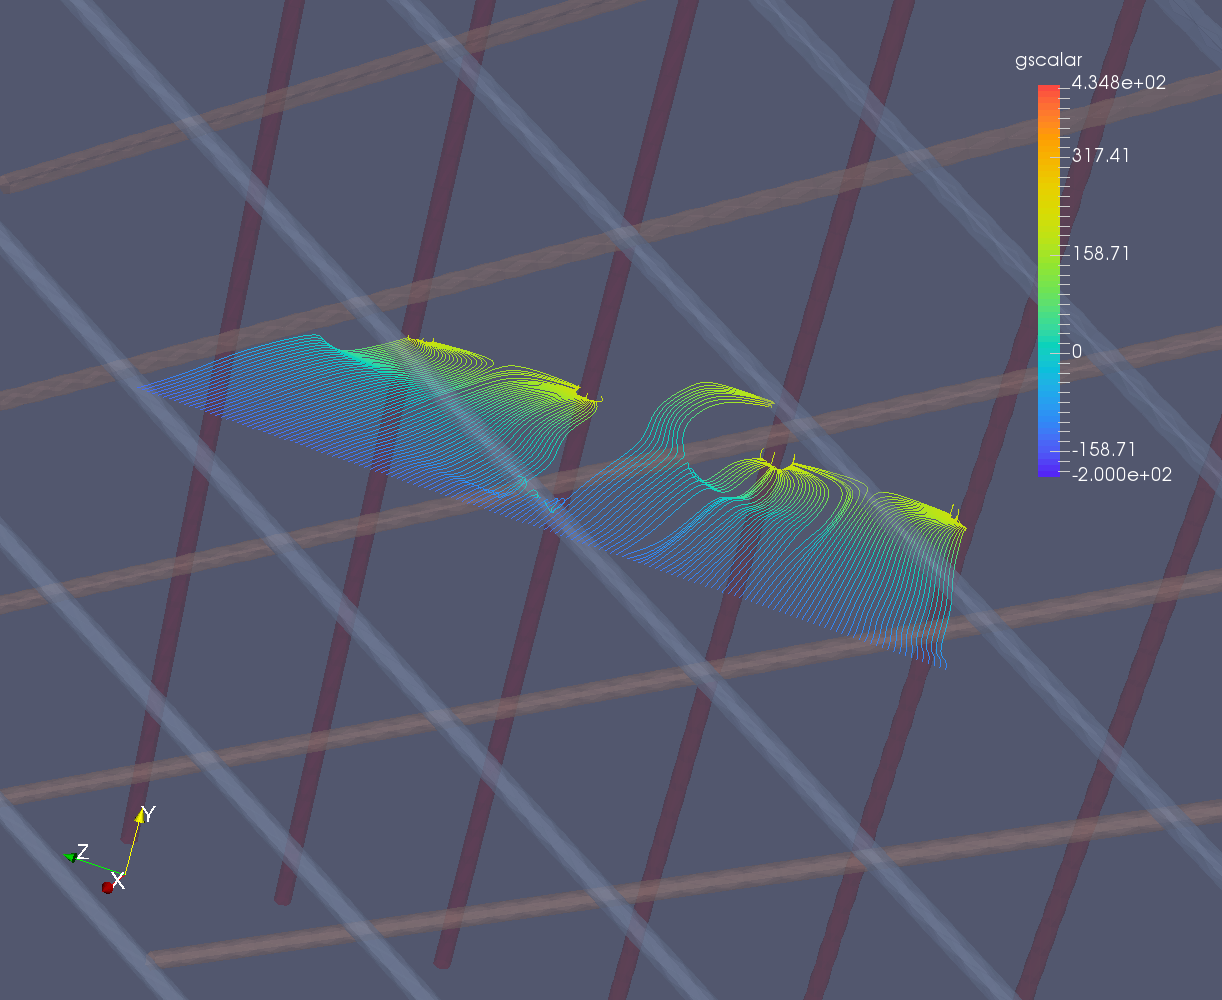
\includegraphics[width=0.7\textwidth]{track-drift-2.png}
  \end{center}
\end{frame}

\section{To Do}

\begin{frame}
  \frametitle{Next steps}

  \begin{itemize}
  \item Compute limitations need some s/w dev workarounds: 
    \begin{itemize}\footnotesize
    \item CPU limited need finer meshing at wire ends, but want
      coarser in middle to save CPU.  Needs a custom mesh alg.
    \item RAM limited: evaluate field in batches over sub-volumes,
      finer grid near surfaces.  
    \end{itemize}
  \item Now have all the pieces for producing response functions, just
    need to bring them all together.
  \item More validation (continuing to collaborate with Leon).
  \item Xin, ``\textit{may need to enlarge problem to +/- 10 wires}''.
    \begin{itemize}\footnotesize
    \item Need to reiterate through the stack of geometry, meshing,
      fields, stepping.  More computing limits expected.
    \end{itemize}
  \end{itemize}

\end{frame}
\end{document}